\documentclass[a4paper,12pt]{report}

% language and encoding
\usepackage{ucs}
\usepackage[utf8x]{inputenc}
\usepackage[english]{babel}

\usepackage{graphicx}
\usepackage{subfigure}
\usepackage{color}
\usepackage{url}

\usepackage{ifthen}

% title
\title{\textbf{Quantum Style Documentation}}

%misc
\author{Saïd Lankri, said.lankri@gmail.com}

% custom commands
\definecolor{darkgreen}{rgb}{0,0.5,0}
\definecolor{darkblue}{rgb}{0,0,0.5}
\definecolor{darkred}{rgb}{0.5,0,0}

\newcommand{\darkred}[1]{\textcolor{red}{#1}}
\newcommand{\green}[1]{\textcolor{darkgreen}{#1}}
\newcommand{\blue}[1]{\textcolor{darkblue}{#1}}

\renewcommand{\thesection}{\arabic{section}}

% MAIN
\begin{document}

\maketitle

\section{What is Quantum Style~?}
QuantumStyle (QS) is an \textbf{SVG} \textbf{themable} style for Qt and KDE
applications.\\

\begin{itemize}
  \item \textbf{Themable} means that the style uses \textbf{themes} to draw
widgets. A widget is a graphical element, like a push button or a combo box. To
draw a widget, the theme looks for the corresponding element in the theme.
You can see a theme as a collection of images, one image is used for push
buttons, another for menus,~... The idea behind using themes is that one can
get different application looks by choosing a theme and without changing the
style. One important difference between themable styles and non themable
styles is that themes can be created by anyone without knowledge of C++
programming, as creating a theme is just a matter of drawing widget elements
and some design.\\

  \item\textbf{SVG} means that themes, that contain elements used to draw
graphical widgets, are stored in the form of SVG files. An SVG file is a
particular type of picture in which you can give names to objets among other
things. SVG files can be created using the open source vector drawing program
\textbf{Inkscape} (\url{http://www.inkscape.org}). In order to use a theme,
each SVG file is associated with a \textbf{theme configuration} file. The SVG
file stores the graphical elements, and the configuration file tells how to use
these elements for widgets.
\end{itemize}

\section{Features}
QS has the following features~:

\begin{itemize}
  \item \textbf{Default theme}. QS has a built-in default theme that is used
when the user has not set any specific theme to use.\\

  \item \textbf{User set theme}. The user can instruct QS to use some
particular theme. The selected theme will be used to draw all widgets of all
applications.\\

  \item \textbf{Per application theme}. In addition to the default and user set
themes, QS can also draw applications with specific themes. This means that you
can use a different theme for each application.

  \item \textbf{Theme Builder}. To help the writing of \textbf{theme
configuration} files, QS comes with a small utility called \textbf{Theme
Builder}. This user friendly tool helps theme designers to easily create and
modify theme configuration files.\\

  \item \textbf{The Debug Mode}. To help theme designers develop their themes,
QS features a \textbf{debug mode}. In this mode, in addition to drawing
widgets, QS adds rectangles with specific colors for various parts of the
widget. Note that debug mode can only be activated at compilation time.
\end{itemize}

\section{How are widgets drawn~?}
$\Rightarrow$ When drawing a widget, the themes looks for the corresponding
elements in the following order~:

\begin{enumerate}
  \item in the \textbf{per application theme} if it exists
  \item in the \textbf{user set theme} if it is set and exists
  \item in the \textbf{default QS theme} which is built-in
\end{enumerate}

$\Rightarrow$ The application name is guessed by calling
\verb,QApplication::applicationName(),\\

\section{Understanding widget drawing}
From QS perspective, \textbf{all} widgets are drawn inside their
\textbf{bounding rect}. They may have a \textbf{frame}, an \textbf{interior},
\textbf{label} specifications and \textbf{indicator} specifications. In
addition, some size related specifications can be set, for instance one can
force a minimal or a fixed size for a widget.\\

$\Rightarrow$ Not all widgets make use of these settings. Basically,
\textbf{all} widgets accept the \textbf{frame} and \textbf{interior} settings.
Widgets that can display text or icons accept the \textbf{label} settings.
Widgets that can display indicators (e.g. tool buttons that can display drop
down arrows) accept the \textbf{indicator} settings.\\

\subsection{Bounding Box}
The bounding box of a widget is the area where the entire widget is drawn.

\begin{figure}[hbtp]
  \centering
  
\includegraphics{bounding-rect.epsi}
\end{figure}

\subsection{Frame}
All widgets can have a \textbf{frame}. The frame is drawn immediately inside the
bounding box with no margins. The \textbf{width} (in pixels) of the frame can be
adjusted for each of the four sides (top, bottom, left, right). The rect
inside the frame is called the \textbf{frame rect}.\\

\begin{figure}[hbtp]
  \centering
  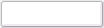
\includegraphics{frame.epsi}
\end{figure}

\subsection{Interior}
All widgets can have an \textbf{interior}. The interior is drawn inside the
\textbf{frame rect} and can have a \textbf{margin}. The rect inside the
interior in called the \textbf{interior rect}.\\

\begin{figure}[hbtp]
  \centering
  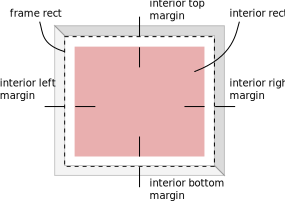
\includegraphics{interior.epsi}
\end{figure}

\subsection{Label}
Widgets that can display text, an icon or both have a \textbf{label}. The label
is drawn inside the \textbf{interior rect} and can have a \textbf{margin}. The
rect inside the label is called the \textbf{label rect}. The spacing between
the icon and the text is called the \textbf{text-icon spacing}.\\

\begin{figure}[hbtp]
  \centering
  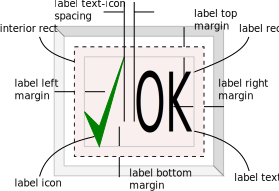
\includegraphics{label.epsi}
\end{figure}

\subsection{Indicator}
Widgets that can display indicators have an \textbf{indicator} setting. The
indicator is drawn inside the \textbf{interior rect} with the same margins as
the label and the same spacing.\\

\begin{figure}[hbtp]
  \centering
  
\includegraphics{indicator.epsi}
\end{figure}

\section{Widget "status"}
QS can draw a widget differently based on its status. There are five supported
statuses~:

\begin{itemize}
  \item "normal". The widget is in a normal status. All but the below.
  \item "focused". The mouse is over the widget. NOTE : the term is misleading,
as we should use "hoovered" or "highlighted".
  \item "pressed". The widget is pressed.
  \item "toggled". For widgets that can be toggled (e.g. tool buttons), the
widget is toggled.
  \item "disabled". The widget is disabled.
\end{itemize}

\textbf{Both} the frame and the interior are drawn based on these statuses
(e.g. a "pressed" widget will be drawn with the "pressed" frame and the
"pressed" interior).

\section{SVG theme design}
Understood widget drawing principles and ready to make your own theme~? Let's
start with an exemple. We want to design a push button.

\subsection{Interior example}
First, we need an SVG file. Let's create one with \textbf{Inkscape} and call it
\verb,myTheme.svg, This SVG file will contain the \textbf{frame} and
\textbf{interior} elements of our push buttons. Remember that for each widget,
QS supports five statuses, so we need five elements for the frame, and five
elements for the interior.\\

To let QS correctly extract these elements to draw a widget, each element must
have a \textbf{name} which obey certain rules. Of course, one can put any other
object in the SVG file. Object which do not obey naming rules or carry
unrecongnized names will be ignored by QS.\\

So let's start by the \textbf{interior}. We need five interiors, like this~:

\begin{figure}[hbtp]
  \centering
  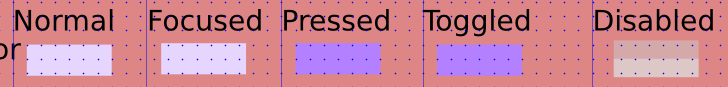
\includegraphics[scale=0.7,angle=-90]{interior-inkscape.epsi}
\end{figure}

\paragraph*{Advice}
\begin{itemize}
  \item An interior can consist of \textbf{several objects}. To make QS able to
use such an interior, you have to \textbf{group} these objects into one object.
Object grouping can be achieved by selecting the desired objects and pressing
\verb,CTRL+G,.\\
  \item Even if your interior consists only of one object, it is a good idea to
group it.\\
  \item In order to "work" inside a group, it is not necessary to ungroup. Just
\textbf{double click} on the object group to \textbf{enter} the group. You'll
now be able to work on indivial objects inside the group. To \textbf{exit} the
group, you have to click on an object which does not belong to the group you're
working on.\\
\end{itemize}

\subsection{SVG Naming Conventions}
Each of the five statuses must obey some naming conventions. for an interior,
QS expects a name in the form \verb,<base>-<status>,.\\

\begin{itemize}
  \item \verb,base, is a basename for the interior that you can set freely. For
example, as we are drawing a push button interior, we can set it to
\verb,button,.\\
  \item \verb,status, is the status of the element. There are five
possibilities~: \verb,normal,, \verb,focused,, \verb,pressed,, \verb,toggled,,
and \verb,disabled,.
\end{itemize}

For example, the element which will be used by QS to draw a normal push button
interior has the name \verb,button-normal,.\\

To \textbf{assign} a name to an element, press \verb,CTRL+SHIFT+o,. A dialog
box will appear. Type in the \textbf{Id} field the name of the element and
don't forget to \textbf{press enter} or click the "set" button.\\

\begin{figure}[hbtp]
  \centering
  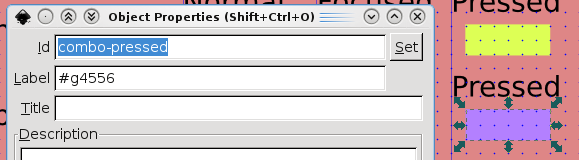
\includegraphics[scale=0.7,angle=-90]{naming.epsi}
\end{figure}

\subsection{Frame example}
As for interiors, we need five frames. But it is a little more complicated.
Each frame consist of eight elements named \verb,<base>-<side>-<status>,. Where
\verb,<base>, is a freely chosen basename, \verb,<side>, is one of \verb,top,,
\verb,bottom,, \verb,left,, \verb,right,, \verb,topleft,, \verb,topright,,
\verb,bottomleft,, \verb,bottomright,, and \verb,<status>, is one of the five
statuses supported by QS.\\

\begin{figure}[hbtp]
  \centering
  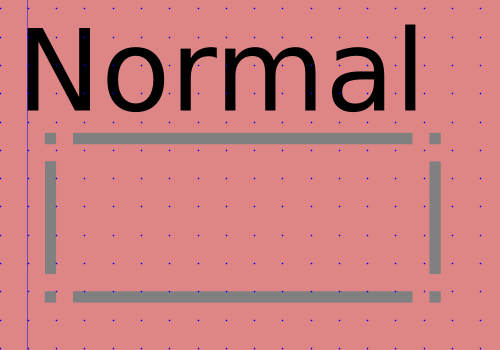
\includegraphics[scale=0.5,angle=-90]{frame-inkscape.epsi}
\end{figure}

It is not possible to simply group these elements as for interiors, because
contrary to interiors, frames must not be stretched when drawn.\\

\subsection{Continuing}
You can apply these steps to draw other elements for widgets. Please note the
following~:

\begin{itemize}
  \item You do not need to draw elements for each type of widget. \textbf{The
same elements} can be reused for multiple widgets. This is specified later in
the theme configuration file.\\

  \item Some widgets have special naming conventions. See the default theme for
an example.
\end{itemize}

\section{Writing a Theme Configuration File}
Once you have designed the svg file, we need a \textbf{theme configuration}
file. If your SVG file is \verb,myTheme.svg, then the theme configuration file
must be named \verb,myTheme.qsconfig,.\\

Theme configuration files are created using the QS theme builder. Launch it and
press "New" button. Give the name \verb,myTheme.qsconfig, and start playing
with the settings. Note that the settings of the default theme are copied to
the newly created theme. On the left you select the widget you to adjust the
settings for, on the right you set the frame, interior, text and indicator
settings. Most important part the the \textbf{basename} setting. This is the
freely chosen name above (without status for interior, without status and side
for frame).

\section{Make QS aware of your theme}
To make QS aware of your theme, some steps are necessary~:

\begin{itemize}
  \item Put both \verb,myTheme.svg, and \verb,myTheme.qsconfig, in a directory
called \verb,myTheme,
  \item Put that directory under \verb,$HOME/.config/QuantumStyle/,
\end{itemize}

To make QS use yout theme, put the line

\begin{verbatim}
theme=myTheme
\end{verbatim}

in the file \verb,$HOME/.config/QuantumStyle/quantumstyle.qsconfig,. This will
instruct QS to use the theme \verb,myTheme, for \textbf{all} applications.

\section{Per application themes}
Making QS aware of a per application theme follows the same procedure as above,
except for the line in \verb,quantumstyle.qsconfig,.\\

If your application name is \verb,konqueror, for example, there must be a
\verb,konqueror, directory in \verb,$HOME/.config/QuantumStyle/, which contains
both \verb,konqueror.svg, and \verb,konqueror.qsconfig,.

\section{Notes}
To avoid any inconsistency, please provide both the SVG and the theme
configuration file.\\
Providing the SVG without the theme configuration file
will lead QS to draw the theme elements using the default configuration
settings.\\
Providing the theme configuration file without the SVG will lead QS to
draw the default elements with the settings of the theme.

\end{document}